% Neural network diagram
% Made with Xematics. Positions are in px (1 px = 0.75 pt), as in the SVG export.
\documentclass[tikz, border=4pt]{standalone}
\definecolor{xm1}{HTML}{FFFFFF}
\definecolor{xm2}{HTML}{1F2937}
\definecolor{xm3}{HTML}{2F7FB5}
\definecolor{xm4}{HTML}{F2F4F6}
\definecolor{xm5}{HTML}{80B1D2}
\definecolor{xm6}{HTML}{6B7280}
\definecolor{xm7}{HTML}{3180B6}
\definecolor{xm8}{HTML}{EAF2F8}
\definecolor{xm9}{HTML}{6BA4CA}
\definecolor{xm10}{HTML}{468DBD}
\definecolor{xm11}{HTML}{E7F0F7}
\definecolor{xm12}{HTML}{CDE0ED}
\definecolor{xm13}{HTML}{ABCBE1}
\definecolor{xm14}{HTML}{84B3D3}
\definecolor{xm15}{HTML}{EAF2F7}
\definecolor{xm16}{HTML}{D5E5F0}
\definecolor{xm17}{HTML}{AACBE1}
\definecolor{xm18}{HTML}{82B2D3}
\definecolor{xm19}{HTML}{BDD6E7}
\definecolor{xm20}{HTML}{E6EFF6}
\definecolor{xm21}{HTML}{ADCDE2}
\definecolor{xm22}{HTML}{3784B8}
\begin{document}
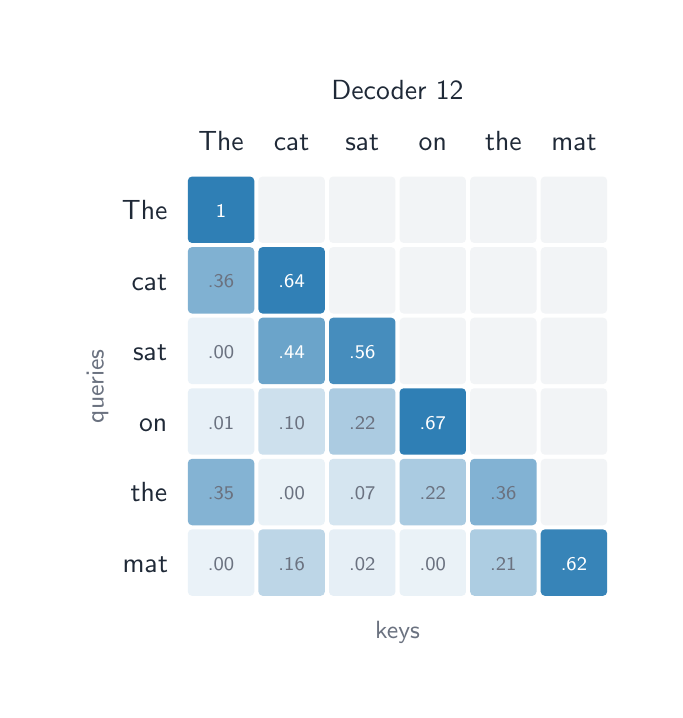
\begin{tikzpicture}[x=0.75pt, y=-0.75pt]
  \tikzset{
    xm text xm2/.style={text=xm2, inner sep=0},
    xm cell nh42b6/.style={fill=xm3, rounded corners=1.5pt},
    xm text xm1/.style={text=xm1, inner sep=0},
    xm cell md7vkh/.style={fill=xm4, rounded corners=1.5pt},
    xm cell l9bots/.style={fill=xm5, rounded corners=1.5pt},
    xm text xm6/.style={text=xm6, inner sep=0},
    xm cell j1jbce/.style={fill=xm7, rounded corners=1.5pt},
    xm cell hxn4lp/.style={fill=xm8, rounded corners=1.5pt},
    xm cell gtqxv0/.style={fill=xm9, rounded corners=1.5pt},
    xm cell 1mvq8zs/.style={fill=xm10, rounded corners=1.5pt},
    xm cell 1lru293/.style={fill=xm11, rounded corners=1.5pt},
    xm cell 1knxvie/.style={fill=xm12, rounded corners=1.5pt},
    xm cell 1jk1orp/.style={fill=xm13, rounded corners=1.5pt},
    xm cell 1ig5i10/.style={fill=xm14, rounded corners=1.5pt},
    xm cell 1hc9bab/.style={fill=xm15, rounded corners=1.5pt},
    xm cell 1g8d4jm/.style={fill=xm16, rounded corners=1.5pt},
    xm cell 1f4gxsx/.style={fill=xm17, rounded corners=1.5pt},
    xm cell 1e0kr28/.style={fill=xm18, rounded corners=1.5pt},
    xm cell 1cwokbj/.style={fill=xm19, rounded corners=1.5pt},
    xm cell oj0g09/.style={fill=xm20, rounded corners=1.5pt},
    xm cell nf499k/.style={fill=xm21, rounded corners=1.5pt},
    xm cell mb82iv/.style={fill=xm22, rounded corners=1.5pt},
  }
  \fill[xm1] (0,0) rectangle (302.18,319.25);
  % Diagram
  \node[xm text xm2, font=\sffamily\fontsize{9.75}{11.7}\selectfont, anchor=base] at (178.18,34.59) {Decoder 12};
  \path[xm cell nh42b6] (77.18,71.73) rectangle ++(32,32);
  \node[xm text xm1, font=\sffamily\fontsize{7.5}{9}\selectfont, anchor=base] at (93.18,91.37) {1};
  \path[xm cell md7vkh] (111.18,71.73) rectangle ++(32,32);
  \path[xm cell md7vkh] (145.18,71.73) rectangle ++(32,32);
  \path[xm cell md7vkh] (179.18,71.73) rectangle ++(32,32);
  \path[xm cell md7vkh] (213.18,71.73) rectangle ++(32,32);
  \path[xm cell md7vkh] (247.18,71.73) rectangle ++(32,32);
  \node[xm text xm2, font=\sffamily\fontsize{9.75}{11.7}\selectfont, anchor=base] at (56.35,92.46) {The};
  \node[xm text xm2, font=\sffamily\fontsize{9.75}{11.7}\selectfont, anchor=base] at (93.18,58.96) {The};
  \path[xm cell l9bots] (77.18,105.73) rectangle ++(32,32);
  \node[xm text xm6, font=\sffamily\fontsize{7.5}{9}\selectfont, anchor=base] at (93.18,125.37) {.36};
  \path[xm cell j1jbce] (111.18,105.73) rectangle ++(32,32);
  \node[xm text xm1, font=\sffamily\fontsize{7.5}{9}\selectfont, anchor=base] at (127.18,125.37) {.64};
  \path[xm cell md7vkh] (145.18,105.73) rectangle ++(32,32);
  \path[xm cell md7vkh] (179.18,105.73) rectangle ++(32,32);
  \path[xm cell md7vkh] (213.18,105.73) rectangle ++(32,32);
  \path[xm cell md7vkh] (247.18,105.73) rectangle ++(32,32);
  \node[xm text xm2, font=\sffamily\fontsize{9.75}{11.7}\selectfont, anchor=base] at (58.62,126.46) {cat};
  \node[xm text xm2, font=\sffamily\fontsize{9.75}{11.7}\selectfont, anchor=base] at (127.18,58.96) {cat};
  \path[xm cell hxn4lp] (77.18,139.73) rectangle ++(32,32);
  \node[xm text xm6, font=\sffamily\fontsize{7.5}{9}\selectfont, anchor=base] at (93.18,159.37) {.00};
  \path[xm cell gtqxv0] (111.18,139.73) rectangle ++(32,32);
  \node[xm text xm1, font=\sffamily\fontsize{7.5}{9}\selectfont, anchor=base] at (127.18,159.37) {.44};
  \path[xm cell 1mvq8zs] (145.18,139.73) rectangle ++(32,32);
  \node[xm text xm1, font=\sffamily\fontsize{7.5}{9}\selectfont, anchor=base] at (161.18,159.37) {.56};
  \path[xm cell md7vkh] (179.18,139.73) rectangle ++(32,32);
  \path[xm cell md7vkh] (213.18,139.73) rectangle ++(32,32);
  \path[xm cell md7vkh] (247.18,139.73) rectangle ++(32,32);
  \node[xm text xm2, font=\sffamily\fontsize{9.75}{11.7}\selectfont, anchor=base] at (58.97,160.46) {sat};
  \node[xm text xm2, font=\sffamily\fontsize{9.75}{11.7}\selectfont, anchor=base] at (161.18,58.96) {sat};
  \path[xm cell 1lru293] (77.18,173.73) rectangle ++(32,32);
  \node[xm text xm6, font=\sffamily\fontsize{7.5}{9}\selectfont, anchor=base] at (93.18,193.37) {.01};
  \path[xm cell 1knxvie] (111.18,173.73) rectangle ++(32,32);
  \node[xm text xm6, font=\sffamily\fontsize{7.5}{9}\selectfont, anchor=base] at (127.18,193.37) {.10};
  \path[xm cell 1jk1orp] (145.18,173.73) rectangle ++(32,32);
  \node[xm text xm6, font=\sffamily\fontsize{7.5}{9}\selectfont, anchor=base] at (161.18,193.37) {.22};
  \path[xm cell nh42b6] (179.18,173.73) rectangle ++(32,32);
  \node[xm text xm1, font=\sffamily\fontsize{7.5}{9}\selectfont, anchor=base] at (195.18,193.37) {.67};
  \path[xm cell md7vkh] (213.18,173.73) rectangle ++(32,32);
  \path[xm cell md7vkh] (247.18,173.73) rectangle ++(32,32);
  \node[xm text xm2, font=\sffamily\fontsize{9.75}{11.7}\selectfont, anchor=base] at (60.44,194.46) {on};
  \node[xm text xm2, font=\sffamily\fontsize{9.75}{11.7}\selectfont, anchor=base] at (195.18,58.96) {on};
  \path[xm cell 1ig5i10] (77.18,207.73) rectangle ++(32,32);
  \node[xm text xm6, font=\sffamily\fontsize{7.5}{9}\selectfont, anchor=base] at (93.18,227.37) {.35};
  \path[xm cell 1hc9bab] (111.18,207.73) rectangle ++(32,32);
  \node[xm text xm6, font=\sffamily\fontsize{7.5}{9}\selectfont, anchor=base] at (127.18,227.37) {.00};
  \path[xm cell 1g8d4jm] (145.18,207.73) rectangle ++(32,32);
  \node[xm text xm6, font=\sffamily\fontsize{7.5}{9}\selectfont, anchor=base] at (161.18,227.37) {.07};
  \path[xm cell 1f4gxsx] (179.18,207.73) rectangle ++(32,32);
  \node[xm text xm6, font=\sffamily\fontsize{7.5}{9}\selectfont, anchor=base] at (195.18,227.37) {.22};
  \path[xm cell 1e0kr28] (213.18,207.73) rectangle ++(32,32);
  \node[xm text xm6, font=\sffamily\fontsize{7.5}{9}\selectfont, anchor=base] at (229.18,227.37) {.36};
  \path[xm cell md7vkh] (247.18,207.73) rectangle ++(32,32);
  \node[xm text xm2, font=\sffamily\fontsize{9.75}{11.7}\selectfont, anchor=base] at (58.42,228.46) {the};
  \node[xm text xm2, font=\sffamily\fontsize{9.75}{11.7}\selectfont, anchor=base] at (229.18,58.96) {the};
  \path[xm cell hxn4lp] (77.18,241.73) rectangle ++(32,32);
  \node[xm text xm6, font=\sffamily\fontsize{7.5}{9}\selectfont, anchor=base] at (93.18,261.37) {.00};
  \path[xm cell 1cwokbj] (111.18,241.73) rectangle ++(32,32);
  \node[xm text xm6, font=\sffamily\fontsize{7.5}{9}\selectfont, anchor=base] at (127.18,261.37) {.16};
  \path[xm cell oj0g09] (145.18,241.73) rectangle ++(32,32);
  \node[xm text xm6, font=\sffamily\fontsize{7.5}{9}\selectfont, anchor=base] at (161.18,261.37) {.02};
  \path[xm cell 1hc9bab] (179.18,241.73) rectangle ++(32,32);
  \node[xm text xm6, font=\sffamily\fontsize{7.5}{9}\selectfont, anchor=base] at (195.18,261.37) {.00};
  \path[xm cell nf499k] (213.18,241.73) rectangle ++(32,32);
  \node[xm text xm6, font=\sffamily\fontsize{7.5}{9}\selectfont, anchor=base] at (229.18,261.37) {.21};
  \path[xm cell mb82iv] (247.18,241.73) rectangle ++(32,32);
  \node[xm text xm1, font=\sffamily\fontsize{7.5}{9}\selectfont, anchor=base] at (263.18,261.37) {.62};
  \node[xm text xm2, font=\sffamily\fontsize{9.75}{11.7}\selectfont, anchor=base] at (56.71,262.46) {mat};
  \node[xm text xm2, font=\sffamily\fontsize{9.75}{11.7}\selectfont, anchor=base] at (263.18,58.96) {mat};
  \node[xm text xm6, font=\sffamily\fontsize{9}{10.8}\selectfont, anchor=base] at (178.18,294.35) {keys};
  \node[xm text xm6, font=\sffamily\fontsize{9}{10.8}\selectfont, anchor=center, rotate=90] at (33.63,172.73) {queries};
\end{tikzpicture}
\end{document}
